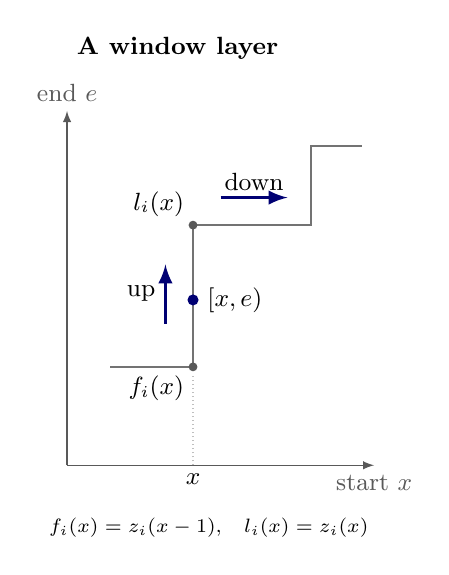
\begin{tikzpicture}[font=\small,>=latex,
  layer/.style={line width=.65pt,draw=black!55},
  connection/.style={line width=1.35pt,draw=blue!45!black},
  guide/.style={draw=black!25,densely dotted,line width=.45pt}]

  \begin{scope}[shift={(0,.75)}]
    \node[anchor=west,font=\small\bfseries] at (0,5.3) {A window layer};
    \draw[->,black!65] (0,0) -- (3.9,0) node[below] {start $x$};
    \draw[->,black!65] (0,0) -- (0,4.5) node[above] {end $e$};
    \draw[layer] (.55,1.25) -- (1.6,1.25) -- (1.6,3.05)
      -- (3.1,3.05) -- (3.1,4.05) -- (3.75,4.05);
    \fill[black!65] (1.6,1.25) circle (1.6pt);
    \fill[black!65] (1.6,3.05) circle (1.6pt);
    \node[anchor=north east,inner sep=3pt] at (1.6,1.25) {$f_i(x)$};
    \node[anchor=south east,inner sep=3pt] at (1.6,3.05) {$l_i(x)$};
    \draw[connection,->] (1.25,1.8) -- (1.25,2.55)
      node[midway,left,inner sep=3pt] {up};
    \draw[connection,->] (1.95,3.4) -- (2.8,3.4)
      node[midway,above,inner sep=2pt] {down};
    \fill[blue!45!black] (1.6,2.1) circle (2pt);
    \node[anchor=west,inner sep=5pt] at (1.6,2.1) {$[x,e)$};
    \draw[guide] (1.6,0) -- (1.6,1.17);
    \node[below,inner sep=3pt] at (1.6,0) {$x$};
    \node[anchor=north,align=center,font=\scriptsize] at (1.8,-.55)
      {$f_i(x)=z_i(x-1)$,\quad $l_i(x)=z_i(x)$};
  \end{scope}

\end{tikzpicture}
